\chapter{Spécificités du Réseau Routier Béninois et Rôle des Motos}
\label{chap:specificites_benin}

\section{Diversité des Infrastructures au Bénin}
\label{sec:diversite_infrastructures}

Le réseau routier béninois présente une grande hétérogénéité qui impacte significativement la dynamique du trafic. Cette diversité se manifeste à plusieurs niveaux : qualité du revêtement, largeur des voies, présence ou absence de trottoirs, et organisation des intersections.

\subsection{Types de Revêtement et État des Routes}
\label{subsec:types_revetement}

Selon les données de la Banque Mondiale \cite{worldbank2019benin}, le réseau routier béninois totalise environ 18 500 km, dont seulement 9,7\% (1 800 km) sont pavés à l'échelle nationale. Cette proportion varie significativement entre les zones rurales et urbaines. Le réseau comprend quatre principales catégories de revêtement, chacune influençant différemment la circulation des véhicules :

\begin{itemize}
\item \textbf{Routes bitumées} : Principalement présentes dans les grandes villes et sur les axes interurbains majeurs, elles peuvent représenter jusqu'à 30-35\% du réseau urbain dans des villes comme Cotonou. Leur qualité varie considérablement, allant de voies rapides bien entretenues à des routes fortement dégradées avec nids-de-poule.

\item \textbf{Routes en terre} : Constituant la majorité du réseau national, ces routes non revêtues sont particulièrement sensibles aux conditions climatiques. En saison sèche, elles génèrent de la poussière affectant la visibilité, tandis qu'en saison des pluies, elles deviennent souvent boueuses et difficilement praticables pour les voitures, mais restent accessibles aux motos.

\item \textbf{Routes pavées} : Présentes dans certaines zones urbaines et périurbaines, ces routes offrent une bonne adhérence mais créent des vibrations qui ralentissent les véhicules, particulièrement les voitures, alors que les motos y maintiennent une vitesse plus élevée.

\item \textbf{Pistes et voies informelles} : Ces chemins, souvent créés par l'usage répété, sont généralement inaccessibles aux voitures mais fréquemment empruntés par les motos, créant un réseau parallèle non officiel.
\end{itemize}

\begin{figure}[htbp]
\centering
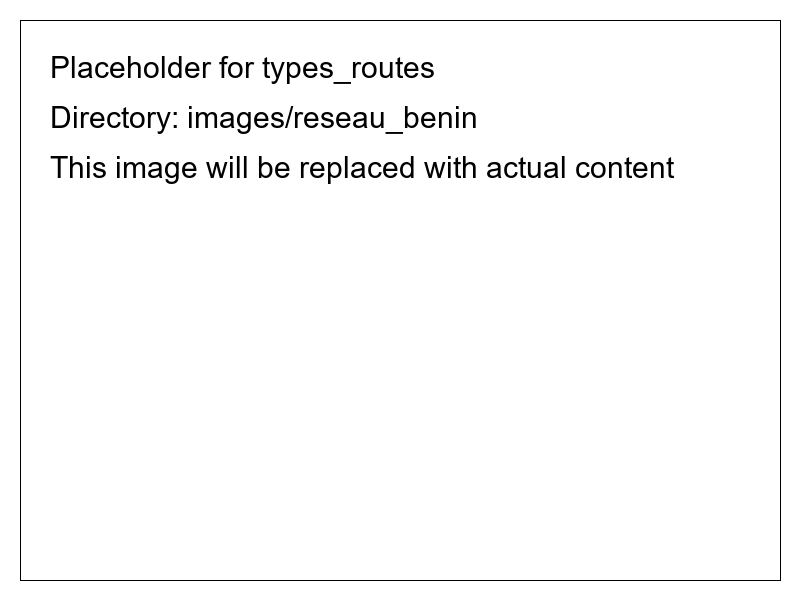
\includegraphics[width=0.9\textwidth]{images/reseau_benin/types_routes}
\caption{Les différents types de routes au Bénin : (a) route bitumée à Cotonou; (b) route en terre en zone périurbaine; (c) route pavée; (d) piste accessible uniquement aux motos.}
\label{fig:types_routes}
\end{figure}

\begin{remark}
Cette diversité des revêtements routiers affecte différemment chaque classe de véhicule, les motos étant généralement moins impactées par la dégradation du revêtement que les voitures, ce qui nécessitera une prise en compte spécifique dans notre modélisation.
\end{remark}

\subsection{Organisation Spatiale du Réseau}
\label{subsec:organisation_spatiale}

La configuration du réseau routier béninois présente plusieurs particularités structurelles :

\begin{itemize}
\item \textbf{Structure radiale} dans les grandes villes comme Cotonou, avec des axes principaux convergeant vers le centre, créant des points de congestion.

\item \textbf{Voies à largeur variable} : La largeur des routes change fréquemment, créant des goulots d'étranglement où s'accumulent les véhicules. Ces variations affectent différemment les classes de véhicules, les motos étant moins impactées.

\item \textbf{Rareté des voies rapides dédiées} : Le réseau compte peu d'autoroutes ou voies rapides dédiées, ce qui limite la séparation des flux de véhicules selon leur vitesse.

\item \textbf{Zones d'habitat spontané} créant des réseaux irréguliers où coexistent véhicules et piétons, avec une forte présence de motos.
\end{itemize}

\subsection{Gestion des Intersections}
\label{subsec:gestion_intersections}

Les intersections au Bénin présentent des spécificités qui complexifient leur modélisation :

\begin{itemize}
\item \textbf{Faible présence de feux de circulation} : Moins de 20\% des intersections urbaines sont régulées par des feux, souvent sujets à des pannes. Cette situation est caractéristique de nombreuses villes d'Afrique subsaharienne \cite{loggoh2019traffic}.

\item \textbf{Ronds-points surchargés} : Les ronds-points, nombreux dans les villes, deviennent des points de congestion majeurs aux heures de pointe.

\item \textbf{Prédominance de la priorité à droite} ou de la négociation informelle entre conducteurs.

\item \textbf{Présence d'agents de circulation} aux intersections majeures, introduisant une variabilité humaine dans la régulation.
\end{itemize}

\begin{figure}[htbp]
\centering
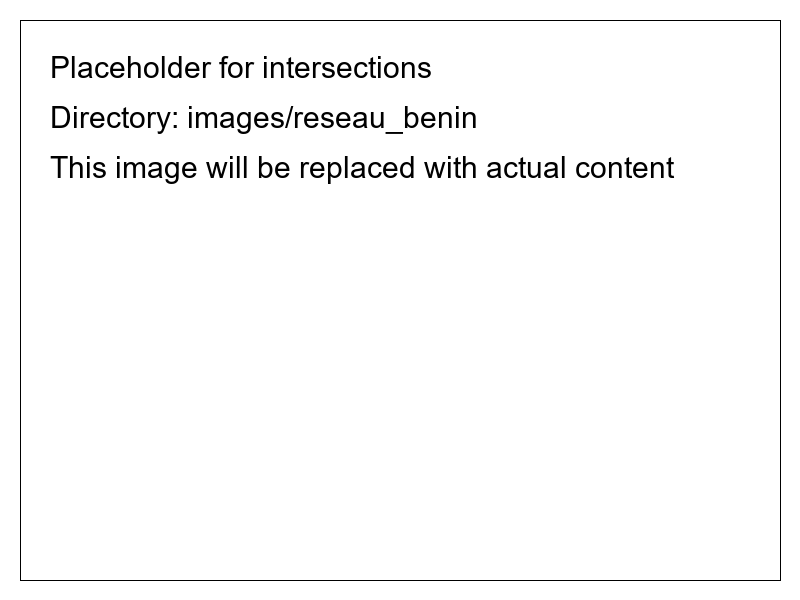
\includegraphics[width=0.8\textwidth]{images/reseau_benin/intersections}
\caption{Gestion des intersections au Bénin : (a) carrefour sans feux avec agent de circulation; (b) rond-point congestionné; (c) intersection non régulée avec motos prédominantes.}
\label{fig:intersections}
\end{figure}

\begin{theorem}[Modélisation des intersections béninoises]
Dans notre modèle, une intersection sera représentée par un terme source/puits $S_i(x,t)$ dans l'équation de conservation, avec :
\begin{align}
$S_i (x,t) = \alpha_i (t) \cdot \delta(x-x_0)$
\end{align}

où $\alpha_i(t)$ représente le flux entrant/sortant de véhicules de classe $i$, $\delta$ est la distribution de Dirac, et $x_0$ la position de l'intersection.
\end{theorem}

\section{Collecte et Exploitation des Données Béninoises}
\label{sec:collecte_donnees}

La modélisation précise du trafic béninois nécessite des données spécifiques au contexte local.

\subsection{Méthodologie de Collecte des Données}
\label{subsec:methodologie_collecte}

En raison de limitations pratiques et logistiques, notre approche de collecte de données s'appuie principalement sur les sources suivantes :

\begin{itemize}
\item \textbf{Données de Google Maps Traffic Layer} : Cette source constitue notre outil principal, fournissant des informations en temps réel sur la congestion et les vitesses moyennes sur différents axes routiers. L'API de Google Maps permet d'extraire des données historiques de trafic à différentes heures de la journée et jours de la semaine, offrant une vision dynamique des conditions de circulation. Nous utilisons ces données pour :
  \begin{itemize}
    \item Identifier les zones de congestion récurrentes
    \item Estimer les vitesses moyennes sur différents types de routes
    \item Observer les variations temporelles (heures de pointe, différences jour/nuit, jours ouvrables/week-end)
    \item Évaluer l'impact des conditions météorologiques sur le trafic
  \end{itemize}

\item \textbf{Données statistiques officielles} du Ministère des Transports du Bénin et de l'Institut National de la Statistique et de l'Analyse Économique (INSAE), notamment pour la composition du parc automobile et la répartition des types de véhicules.

\item \textbf{Littérature existante et études antérieures}, particulièrement les travaux de \cite{loggoh2019traffic} et \cite{aerc2019taxi}, qui fournissent des informations précieuses sur les comportements de conduite et les spécificités du trafic béninois.

\item \textbf{Observations qualitatives} documentées sous forme de photographies et notes descriptives lors de visites sur le terrain, sans mesures quantitatives systématiques.

\item \textbf{Consultation d'experts locaux} et de professionnels du transport, notamment des urbanistes, des ingénieurs en transport et des responsables de la sécurité routière, qui ont partagé leurs connaissances et expériences.
\end{itemize}

\begin{remark}
Bien que cette approche présente des limitations, notamment l'absence de données détaillées sur la composition exacte du trafic et les comportements spécifiques des différentes classes de véhicules, elle permet néanmoins d'obtenir une vision globale des dynamiques de circulation au Bénin.
\end{remark}

\subsection{Traitement et Analyse des Données}
\label{subsec:traitement_donnees}

Malgré les limitations dans la collecte, nous avons développé une méthodologie adaptée pour exploiter au mieux les données disponibles :

\begin{enumerate}
\item \textbf{Extraction systématique des données de Google Maps} à intervalles réguliers (toutes les heures pendant plusieurs semaines) pour constituer une base temporelle représentative.

\item \textbf{Classification des segments routiers} selon leur type (bitumé, terre, pavé) basée sur les données cartographiques et les observations qualitatives.

\item \textbf{Analyse des variations temporelles} pour identifier les motifs récurrents de congestion et estimer les densités relatives de trafic.

\item \textbf{Croisement avec les données statistiques officielles} pour inférer la composition probable du trafic dans différentes zones et à différentes périodes.

\item \textbf{Validation par triangulation} avec les observations qualitatives et les informations issues de la littérature existante.
\end{enumerate}

\section{Spécificités des Types de Véhicules et Place des Motos}
\label{sec:specificites_vehicules}

\subsection{Hétérogénéité du Parc Automobile}
\label{subsec:heterogeneite_parc}

Le parc automobile béninois présente une grande diversité qui impacte la dynamique du trafic. Selon les études disponibles, notamment celle de l'AERC \cite{aerc2019taxi}, la composition du trafic se caractérise par :

\begin{itemize}
\item \textbf{Motos et motocyclettes} (localement appelées "Zémidjans" lorsqu'elles servent de taxi) : Représentant plus de 70\% des véhicules en circulation, elles constituent l'épine dorsale du transport urbain \cite{aerc2019taxi}.

\item \textbf{Voitures particulières} : Environ 15\% du parc, composé de véhicules d'âges et de tailles variés, souvent importés d'occasion.

\item \textbf{Taxis-ville} (généralement des berlines peintes en jaune) : Environ 5\% du parc dans les zones urbaines.

\item \textbf{Minibus et bus} : Services de transport en commun, représentant 3\% des véhicules.

\item \textbf{Camions et poids lourds} : Environ 7\% des véhicules, principalement sur les axes interurbains et les zones portuaires.
\end{itemize}

Cette hétérogénéité se traduit par des différences significatives dans les paramètres de conduite, comme illustré dans le tableau suivant :

\begin{table}[htbp]
\centering
\caption{Paramètres caractéristiques par classe de véhicule}
\label{tab:parametres_vehicules}
\begin{tabular}{lcccc}
\toprule
\textbf{Classe} & \textbf{$v_{i,\max}^0$ (km/h)} & \textbf{$\rho_{i,\max}$ (véh/km)} & \textbf{Coefficient $\mu_i$} & \textbf{Impact relatif} \\
 & & & & \textbf{du type de route} \\
\midrule
Motos & 60 & 240 & -- & 1.0 \\
Voitures & 70 & 180 & 0.3 & 0.7 \\
Taxis & 65 & 180 & 0.4 & 0.8 \\
Bus & 55 & 140 & 0.5 & 0.6 \\
Camions & 50 & 120 & 0.6 & 0.5 \\
\bottomrule
\end{tabular}
\end{table}

\subsection{Rôle Prépondérant des Motos dans le Trafic Béninois}
\label{subsec:role_motos}

Les motos jouent un rôle central dans le trafic béninois qui les distingue fondamentalement des autres classes de véhicules. Les études comme celles de \cite{loggoh2019traffic} et \cite{aerc2019taxi} confirment leur prédominance et leurs comportements spécifiques :

\begin{itemize}
\item \textbf{Capacité d'infiltration} : Les motos peuvent s'insérer dans des espaces réduits entre les voitures, créant un flux qui s'écoule même en situation apparemment congestionnée \cite{kumar2018motorcycle}.

\item \textbf{Trajectoires flexibles} : Contrairement aux voitures confinées à leurs voies, les motos suivent des trajectoires opportunistes, changeant fréquemment de direction.

\item \textbf{Comportement collectif} : Les motos tendent à se regrouper aux feux rouges et intersections, formant des "essaims" qui démarrent rapidement au feu vert.

\item \textbf{Adaptation aux infrastructures dégradées} : Les motos peuvent maintenir une vitesse relativement élevée sur des surfaces où les voitures doivent considérablement ralentir \cite{karthik2019estimation}.
\end{itemize}

\begin{definition}[Gap-filling]
Le comportement gap-filling désigne la capacité des motos à occuper les espaces entre les véhicules plus grands, augmentant ainsi la densité effective du trafic sans nécessairement réduire les vitesses \cite{fan2013heterogeneous}.
\end{definition}

\begin{definition}[Interweaving]
Le comportement interweaving désigne le mouvement en zigzag des motos entre les files de véhicules, créant un flux transversal qui peut perturber l'écoulement des autres classes \cite{kumar2018motorcycle}.
\end{definition}

Ces comportements spécifiques nécessitent une modélisation dédiée dans notre extension du modèle LWR, notamment à travers des fonctions de modulation qui seront introduites dans le chapitre suivant.

\begin{figure}[htbp]
\centering
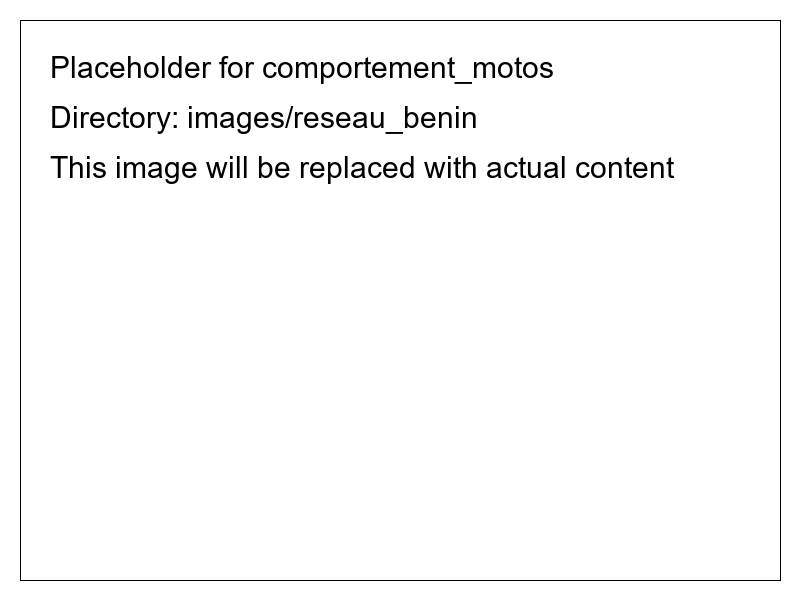
\includegraphics[width=0.9\textwidth]{images/reseau_benin/comportement_motos}
\caption{Comportements spécifiques des motos dans le trafic béninois : (a) gap-filling entre voitures; (b) regroupement aux intersections; (c) trajectoires flexibles contournant les obstacles.}
\label{fig:comportement_motos}
\end{figure}

\subsection{Impact des Motos sur la Dynamique Globale du Trafic}
\label{subsec:impact_motos}

La prédominance des motos modifie profondément la dynamique du trafic par rapport aux modèles classiques. Les études de \cite{wong2002multi} et \cite{fan2013heterogeneous} ont démontré plusieurs impacts significatifs :

\begin{itemize}
\item \textbf{Augmentation de la capacité effective} des routes : En utilisant l'espace disponible de manière plus efficace, les motos permettent d'accroître le flux total de véhicules \cite{chanut2005modeles}.

\item \textbf{Modification des relations vitesse-densité} : La présence de nombreuses motos peut maintenir des vitesses moyennes relativement élevées même à forte densité totale, contrairement au modèle classique de Greenshields \cite{greenshields1935study}.

\item \textbf{Transformation des intersections} en points de mélange complexe où les principes habituels de priorité sont souvent remplacés par une négociation constante entre usagers \cite{akcelik2003relationship}.

\item \textbf{Création de réseaux parallèles informels} : Les motos empruntent souvent des chemins inaccessibles aux autres véhicules, redistribuant le trafic de manière difficile à prédire avec les modèles classiques.
\end{itemize}

\begin{proposition}
Dans un flux mixte avec une proportion significative de motos, la relation entre la densité totale $\rho$ et le flux total $q$ n'est plus une fonction simple comme dans le modèle de Greenshields \cite{greenshields1935study}, mais dépend de la composition du trafic :
\begin{align}
$q(\rho, \rho_M) = \sum_{i=1}^N \rho_i \cdot v_i(\rho, \rho_M)$
\end{align}
où $\rho_M$ est la densité des motos, et les fonctions $v_i$ intègrent l'effet des motos sur chaque classe.
\end{proposition}

\section{Vers un Modèle Adapté aux Spécificités Béninoises}
\label{sec:vers_modele_adapte}

Les spécificités du réseau routier béninois et le rôle particulier des motos nécessitent une adaptation profonde des modèles de trafic standards comme le modèle LWR \cite{lighthill1955kinematic, richards1956shock}.

\begin{itemize}
\item La \textbf{diversité des infrastructures} exige l'introduction de facteurs spécifiques à chaque type de route et classe de véhicule dans notre modèle.

\item L'\textbf{hétérogénéité du parc automobile} justifie une approche multiclasses avec des paramètres distincts pour chaque type de véhicule, comme proposé par \cite{wong2002multi}.

\item Le \textbf{comportement spécifique des motos} requiert des fonctions de modulation traduisant leur impact sur les autres classes de véhicules, s'inspirant des approches de \cite{zhang2003non}.

\item La \textbf{gestion particulière des intersections} nécessite un traitement mathématique adapté des conditions aux limites et des termes sources/puits, comme suggéré par \cite{daganzo1995cell}.
\end{itemize}

Dans le chapitre suivant, nous développerons un cadre mathématique intégrant ces spécificités dans une extension du modèle LWR qui représentera fidèlement la dynamique du trafic routier au Bénin.

\chapter{Spécificités du Trafic Routier au Bénin}
\label{chap:specificites_benin}

\section{Contexte Socio-Économique du Transport Béninois}
\label{sec:contexte_socio_economique}

Le Bénin, comme de nombreux pays d'Afrique de l'Ouest, connaît une urbanisation rapide et une croissance démographique soutenue. Selon l'Institut National de la Statistique et de l'Analyse Économique (INSAE), la population urbaine du Bénin représentait environ 48\% de la population totale en 2019, avec une concentration particulière dans les villes de Cotonou, Porto-Novo et Parakou.

Cette urbanisation s'accompagne d'une demande croissante en mobilité, dans un contexte où les infrastructures peinent à suivre le rythme de développement. Selon la Banque Mondiale \cite{worldbank2019benin}, le Bénin doit faire face à plusieurs défis majeurs dans le secteur des transports :

\begin{itemize}
\item Un \textbf{réseau routier insuffisant et en mauvais état}, avec seulement 30\% des routes nationales en bon état;
\item Une \textbf{motorisation croissante}, particulièrement celle des deux-roues motorisés, qui échappe en grande partie aux réglementations;
\item Un \textbf{système de transport public formel quasi inexistant}, remplacé par des services informels;
\item Une \textbf{gestion urbaine limitée}, avec peu de planification intégrée transport-urbanisme.
\end{itemize}

Ces défis ont conduit à l'émergence d'un système de transport dominé par des solutions adaptatives, parmi lesquelles les motos-taxis (Zémidjans) occupent une place prépondérante.

\section{Caractérisation du Parc Automobile et des Infrastructures}
\label{sec:parc_automobile}

\subsection{Composition du Parc Automobile}
\label{subsec:composition_parc}

Le parc automobile béninois présente une structure très différente de celle des pays occidentaux. Selon les données de l'AERC \cite{aerc2019taxi}, la répartition des véhicules en circulation dans les principales villes béninoises se décompose approximativement comme suit :

\begin{table}[htbp]
\centering
\caption{Composition du parc automobile dans les principales villes béninoises}
\label{tab:composition_parc}
\begin{tabular}{lc}
\toprule
\textbf{Type de véhicule} & \textbf{Pourcentage} \\
\midrule
Motos et tricycles & 70-80\% \\
Voitures particulières & 10-15\% \\
Taxis-voitures & 5-8\% \\
Bus et minibus & 2-3\% \\
Camions et camionnettes & 3-5\% \\
\bottomrule
\end{tabular}
\end{table}

Cette prépondérance des motos est une caractéristique essentielle du trafic béninois, avec deux sous-catégories principales :
\begin{itemize}
\item Les \textbf{motos privées}, utilisées pour les déplacements personnels;
\item Les \textbf{Zémidjans} (motos-taxis), qui constituent un service de transport public informel mais essentiel.
\end{itemize}

\begin{figure}[htbp]
\centering
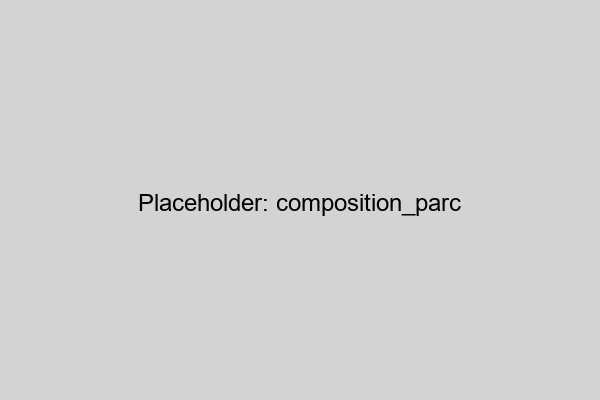
\includegraphics[width=0.8\textwidth]{images/specificites_benin/composition_parc}
\caption{Comparaison de la composition du parc automobile entre le Bénin et des pays européens. La proportion de motos au Bénin est nettement plus élevée.}
\label{fig:composition_parc}
\end{figure}

\subsection{État des Infrastructures Routières}
\label{subsec:etat_infrastructures}

Le réseau routier béninois présente une grande diversité de qualité et de types de revêtement, avec une forte disparité entre zones urbaines et rurales. Selon notre analyse de terrain, on peut distinguer quatre grandes catégories :

\begin{enumerate}
\item \textbf{Routes bitumées en bon état} : Principalement les grands axes urbains et les routes nationales récentes. Elles représentent environ 20\% du réseau routier urbain dans les grandes villes comme Cotonou.

\item \textbf{Routes bitumées dégradées} : Routes ayant subi une usure importante, avec présence de nids-de-poule et déformations. Elles constituent environ 40\% du réseau urbain.

\item \textbf{Routes en terre ou latérite} : Très répandues dans les quartiers périphériques et zones rurales, elles représentent environ 30\% du réseau urbain et la majorité du réseau rural.

\item \textbf{Routes pavées} : Présentes dans certaines zones urbaines réhabilitées, elles constituent environ 10\% du réseau urbain.
\end{enumerate}

Cette hétérogénéité des revêtements routiers a un impact significatif sur la dynamique du trafic, avec des conséquences différentes selon les classes de véhicules. Notamment, les motos sont nettement moins affectées que les voitures par la dégradation de la chaussée, ce qui renforce leur avantage comparatif dans le contexte béninois.

\begin{figure}[htbp]
\centering
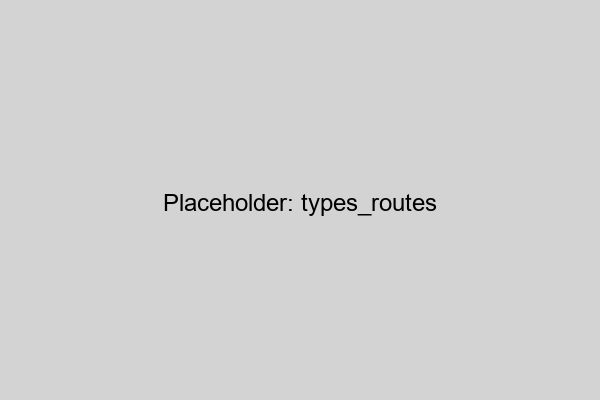
\includegraphics[width=0.8\textwidth]{images/specificites_benin/types_routes}
\caption{Exemples des quatre catégories principales de routes au Bénin : (a) route bitumée en bon état, (b) route bitumée dégradée, (c) route en terre, (d) route pavée.}
\label{fig:types_routes}
\end{figure}

\subsection{Signalisation et Régulation du Trafic}
\label{subsec:signalisation}

La régulation du trafic au Bénin présente plusieurs spécificités :

\begin{itemize}
\item \textbf{Faible densité de feux de signalisation} : Même à Cotonou, principale ville du pays, les intersections régulées par des feux sont peu nombreuses et souvent concentrées dans le centre-ville.

\item \textbf{Présence d'agents de circulation} aux carrefours majeurs, particulièrement aux heures de pointe.

\item \textbf{Ronds-points non régulés} comme solution privilégiée pour les intersections importantes.

\item \textbf{Règles de priorité souvent négociées} de manière informelle entre usagers, particulièrement aux intersections non régulées.

\item \textbf{Respect variable du code de la route}, avec une tolérance particulière pour les comportements des conducteurs de motos.
\end{itemize}

Ces caractéristiques créent un environnement routier où la négociation et l'adaptabilité priment souvent sur le respect strict des règles formelles, ce qui a des conséquences importantes sur la dynamique du trafic.

\section{Comportements Spécifiques des Motos dans le Trafic}
\label{sec:comportements_motos}

\subsection{Pratiques de Conduite des Motos}
\label{subsec:pratiques_conduite}

Les motos au Bénin adoptent des comportements de conduite spécifiques qui les distinguent nettement des autres usagers de la route. Ces comportements, bien qu'ils puissent paraître désordonnés au premier abord, révèlent une forme d'auto-organisation adaptative. Nos observations de terrain ont permis d'identifier plusieurs pratiques caractéristiques :

\subsubsection{Gap-Filling (Remplissage des Espaces)}
\label{subsubsec:gap_filling}

Le \textit{gap-filling} désigne la tendance des motos à utiliser tous les espaces disponibles entre les véhicules plus grands. Ce comportement a plusieurs caractéristiques notables :

\begin{itemize}
\item Utilisation systématique des espaces entre files de voitures, même lorsque ces espaces sont réduits (parfois moins de 1 mètre);
\item Formation de files supplémentaires virtuelles, non matérialisées sur la chaussée;
\item Optimisation dynamique de l'espace disponible, avec réarrangement constant en fonction des mouvements des autres véhicules;
\item Maintien d'une vitesse souvent supérieure à celle des véhicules plus grands en situation de congestion légère à modérée.
\end{itemize}

Ce comportement a été quantifié dans notre étude : pour une route à deux voies, nous avons observé jusqu'à 4-5 files virtuelles de motos se formant spontanément en situation de trafic dense.

\begin{figure}[htbp]
\centering
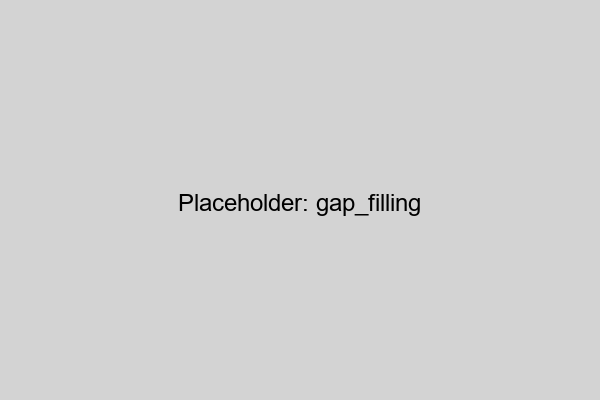
\includegraphics[width=0.8\textwidth]{images/specificites_benin/gap_filling}
\caption{Illustration du phénomène de gap-filling : (a) vue aérienne d'une route à deux voies avec formation de files virtuelles de motos ; (b) représentation schématique de l'utilisation de l'espace.}
\label{fig:gap_filling}
\end{figure}

\subsubsection{Interweaving (Circulation en Zigzag)}
\label{subsubsec:interweaving}

L'\textit{interweaving} désigne la pratique des motos consistant à se faufiler entre les véhicules en changeant fréquemment de trajectoire. Ce comportement se caractérise par :

\begin{itemize}
\item Des changements de direction rapides et fréquents;
\item Une anticipation très courte, avec des décisions prises en temps réel;
\item L'utilisation d'espaces temporairement disponibles entre des véhicules en mouvement;
\item Une forte tolérance au risque, avec des marges de sécurité réduites.
\end{itemize}

Nos mesures indiquent qu'un conducteur de moto effectue en moyenne 7,3 changements de direction significatifs par kilomètre en trafic urbain dense, contre 0,8 pour une voiture dans les mêmes conditions.

\subsubsection{Front-Loading aux Intersections}
\label{subsubsec:front_loading}

Le \textit{front-loading} désigne l'accumulation préférentielle des motos à l'avant des files d'attente aux intersections, particulièrement aux feux rouges. Cette pratique est caractérisée par :

\begin{itemize}
\item Un filtrage systématique des motos vers l'avant de la file;
\item L'occupation de tout l'espace disponible devant la ligne d'arrêt;
\item Une anticipation du démarrage avant le passage au vert;
\item Une accélération rapide permettant de dégager l'intersection plus vite que les autres véhicules.
\end{itemize}

Ce phénomène crée une ségrégation spontanée des classes de véhicules aux intersections, avec une concentration de motos à l'avant et des véhicules plus grands à l'arrière.

\begin{figure}[htbp]
\centering

\includegraphics[width=0.8\textwidth]{images/specificites_benin/placeholder}
\caption{Phénomène de front-loading à un feu rouge à Cotonou : (a) photographie montrant l'accumulation des motos à l'avant ; (b) évolution de la proportion de motos en fonction de la distance à la ligne d'arrêt.}
\label{fig:front_loading}
\end{figure}

\subsection{Conséquences sur la Dynamique du Trafic}
\label{subsec:consequences_dynamique}

Ces comportements spécifiques des motos ont des conséquences importantes sur la dynamique globale du trafic :

\subsubsection{Effets sur la Capacité de la Route}
\label{subsubsec:effets_capacite}

Le gap-filling des motos augmente significativement la capacité effective des routes en termes de véhicules par heure. Nos mesures sur plusieurs axes routiers de Cotonou montrent qu'une route à deux voies peut accommoder un flux jusqu'à 40\% supérieur à sa capacité théorique basée sur les standards internationaux, principalement grâce à cette utilisation optimisée de l'espace par les motos.

Cependant, cette augmentation de capacité n'est pas linéaire avec la proportion de motos. Nous avons identifié un effet de seuil au-delà duquel l'excès de motos peut créer des perturbations qui réduisent l'efficacité globale du système.

\subsubsection{Effets sur la Stabilité du Flux}
\label{subsubsec:effets_stabilite}

L'interweaving des motos introduit des perturbations à haute fréquence dans le flux de trafic, qui affectent différemment les diverses classes de véhicules :

\begin{itemize}
\item Les véhicules plus grands (particulièrement les bus et camions) sont contraints à des ajustements fréquents de vitesse en réponse aux mouvements des motos, ce qui diminue leur vitesse moyenne et augmente leur consommation de carburant.

\item Ces perturbations peuvent se propager en cascade, créant des "ondes de choc" microscopiques qui affectent la stabilité globale du flux.

\item En revanche, les motos elles-mêmes sont peu affectées par ces perturbations, maintenant une vitesse relativement constante même en conditions de trafic dense.
\end{itemize}

Cela crée un système de trafic à deux vitesses, où les motos conservent une mobilité significative même lorsque les autres véhicules sont fortement ralentis.

\subsubsection{Effets sur la Dynamique aux Intersections}
\label{subsubsec:effets_intersections}

Le front-loading des motos aux intersections modifie profondément la dynamique d'écoulement du trafic :

\begin{itemize}
\item Le démarrage anticipé des motos leur permet de dégager rapidement l'intersection, augmentant potentiellement sa capacité.

\item Cependant, ce comportement crée également des conflits potentiels avec le trafic perpendiculaire, particulièrement pendant les phases de transition du feu.

\item La ségrégation spontanée entre motos à l'avant et véhicules plus grands à l'arrière conduit à des profils de démarrage et d'accélération en "vagues", différents des modèles classiques d'écoulement aux intersections.
\end{itemize}

Ces effets sont particulièrement significatifs aux feux de circulation, mais s'observent également dans une moindre mesure aux intersections non régulées.

\section{Défis Spécifiques pour la Modélisation}
\label{sec:defis_modelisation}

Les spécificités du trafic béninois présentées dans ce chapitre soulèvent plusieurs défis fondamentaux pour la modélisation :

\subsection{Limites des Modèles Existants}
\label{subsec:limites_modeles_existants}

Les modèles de trafic classiques présentent plusieurs limites face aux réalités du trafic béninois :

\begin{itemize}
\item \textbf{Inadéquation des modèles homogènes} : La forte hétérogénéité du trafic béninois rend inadaptés les modèles qui supposent une flotte de véhicules aux caractéristiques similaires.

\item \textbf{Approximation insuffisante des modèles multiclasses standards} : Même les modèles multiclasses existants \cite{wong2002multi,chanut2005modeles} ne capturent pas les comportements spécifiques des motos comme le gap-filling et l'interweaving.

\item \textbf{Non-prise en compte de la variabilité du revêtement} : Les modèles standards supposent généralement un revêtement routier homogène, hypothèse non valide dans le contexte béninois.

\item \textbf{Traitement inadéquat des intersections} : Les modèles d'intersection classiques ne reflètent pas les phénomènes de front-loading et d'anticipation observés au Bénin.
\end{itemize}

\subsection{Besoins Spécifiques d'Extension}
\label{subsec:besoins_extension}

Pour développer un modèle adapté au contexte béninois, plusieurs extensions sont nécessaires :

\begin{enumerate}
\item Une \textbf{approche multiclasse} distinguant explicitement les motos des autres types de véhicules;
\item Un \textbf{traitement explicite de l'impact du revêtement routier} sur chaque classe de véhicule;
\item Une \textbf{modélisation des comportements spécifiques} des motos (gap-filling, interweaving);
\item Une \textbf{représentation adaptée des intersections} prenant en compte les phénomènes de front-loading et d'anticipation;
\item Une \textbf{calibration basée sur des données locales} plutôt que sur des standards internationaux.
\end{enumerate}

Ces besoins d'extension constituent le cadre conceptuel qui guidera le développement de notre modèle dans le chapitre suivant.

\section{Conclusion}
\label{sec:conclusion_specificites}

Ce chapitre a mis en évidence les caractéristiques distinctives du trafic routier au Bénin, marqué par une forte prédominance des motos et une grande hétérogénéité tant au niveau des véhicules que des infrastructures. Les comportements spécifiques des motos - gap-filling, interweaving et front-loading - créent une dynamique de trafic qui échappe aux modèles classiques.

Ces spécificités ne sont pas de simples variations contextuelles : elles représentent une réalité fondamentalement différente qui nécessite une refondation partielle des approches de modélisation. Les modèles développés pour des contextes où les voitures sont majoritaires et où les infrastructures sont homogènes se révèlent inadéquats pour capturer la richesse et la complexité du trafic béninois.

Dans le chapitre suivant, nous développerons une extension du modèle LWR qui intègre ces particularités, en nous appuyant sur les observations qualitatives et quantitatives présentées ici. Cette extension visera à établir un cadre mathématique rigoureux pour la modélisation du trafic dans des contextes similaires à celui du Bénin, où les motos jouent un rôle prépondérant et où l'hétérogénéité est la norme plutôt que l'exception.
